\section{Loading data}
\paragraph{}
For our following experiments, we will use the following textures:
\begin{figure}[h]
    \centering
    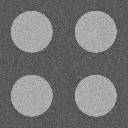
\includegraphics[scale=0.6]{rdf-2-classes-texture-0.png}
    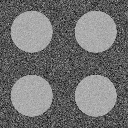
\includegraphics[scale=0.6]{rdf-2-classes-texture-1.png}
    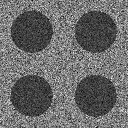
\includegraphics[scale=0.6]{rdf-2-classes-texture-2.png}
    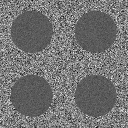
\includegraphics[scale=0.6]{rdf-2-classes-texture-3.png}
    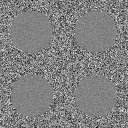
\includegraphics[scale=0.6]{rdf-2-classes-texture-4.png}
    \caption{Images to experiment on}
\end{figure}

\paragraph{}
Our reference image (having a clear difference between objects and background) is the following:
\begin{figure}[h]
    \centering
    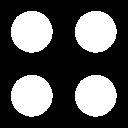
\includegraphics[scale=0.6]{rdf-masque-ronds.png}
    \caption{Reference image}
    \label{fig-reference-image}
\end{figure}

\paragraph{}
These will be loaded and converted to gray images:
\begin{lstlisting}[language=R, caption=Loading images]
    rdfReadGreyImage <- function (nom) {
        image <- readImage (nom)
        if (length (dim (image)) == 2) {
            image
        } else {
            channel (image, 'red')
        }
    }
\end{lstlisting}

\clearpage

\section{Gray levels}
\subsection{Gray values histogram}
\paragraph{}
A first good step would be taking a look at how the gray values are distributed. We can use a \emph{histogram} for this.
\begin{lstlisting}[language=R, caption=Creating histograms of gray values]
    buildHistogram <- function (nom, nbins){
        image <- rdfReadGreyImage (nom)
        h <- hist (as.vector (image), breaks = seq (0, 1, 1 / nbins), main = nom)
    }
\end{lstlisting}

\begin{figure}[h]
    \centering
    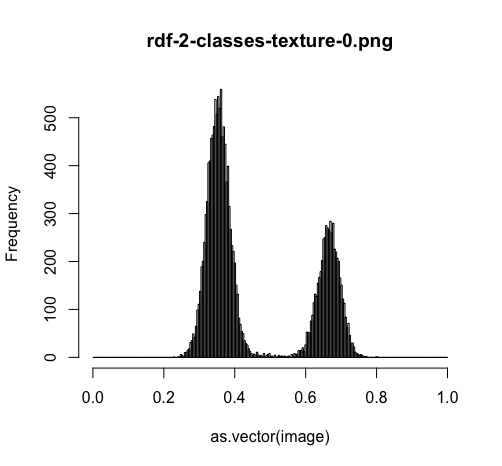
\includegraphics[width=\textwidth/3]{gray_values_0.png}
    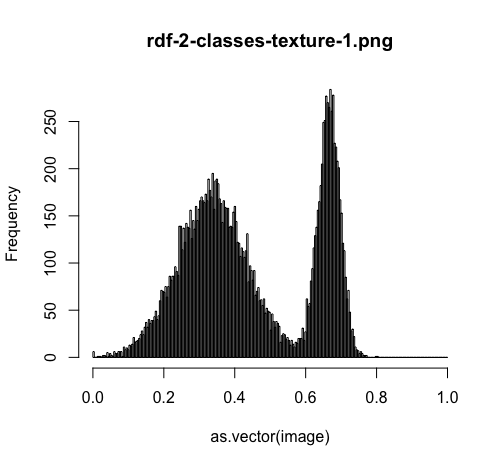
\includegraphics[width=\textwidth/3]{gray_values_1.png}
    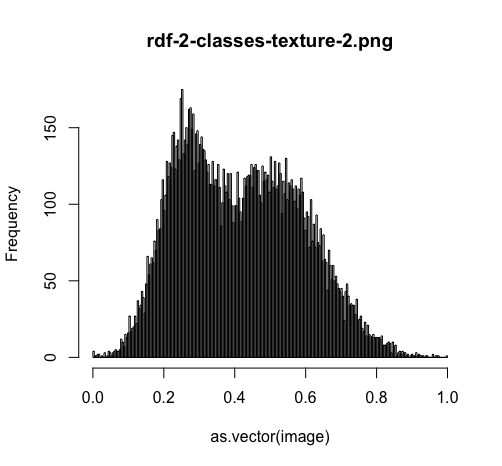
\includegraphics[width=\textwidth/3]{gray_values_2.png}
    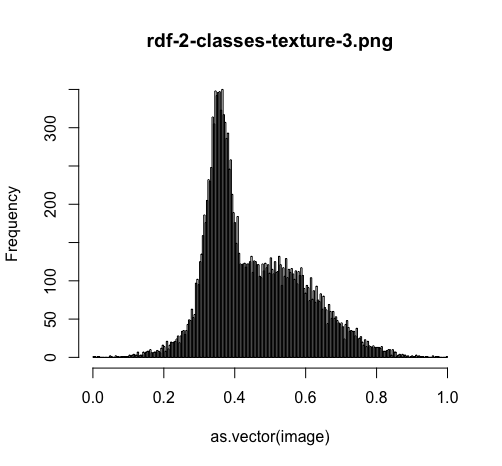
\includegraphics[width=\textwidth/3]{gray_values_3.png}
    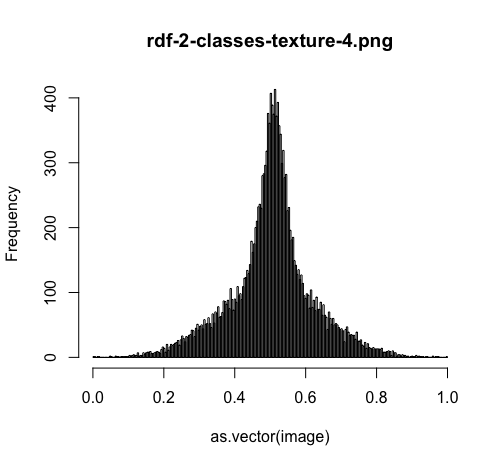
\includegraphics[width=\textwidth/3]{gray_values_4.png}
    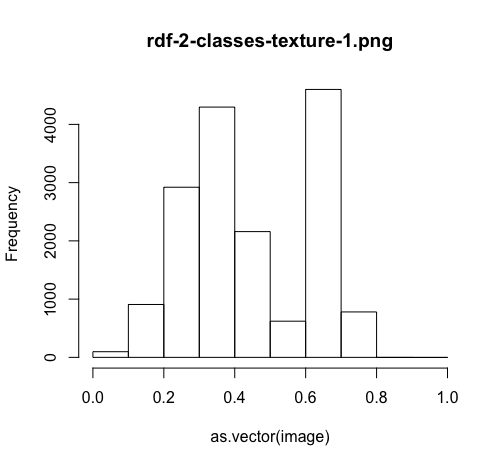
\includegraphics[width=\textwidth/3]{histogram_10bins.png}
    \caption{Histograms of gray values}
    \label{fig-histograms}
\end{figure}

\paragraph{}
Since each pixel can have a gray value from $0$ to $255$, we therefore have a total number of $256$ values, so that is going to be our number of \emph{bins} for the histogram.
If we were to use, for example, only $10$ bins, that would give the number of pixels with gray values between $[0, 0.1)$, $[0.1, 0.2)$ and so on, as it can be seen in the last image \ref{fig-histograms}.

\subsection{Thresholding based on gray values}
\paragraph{}
Based on the histograms above \ref{fig-histograms}, we may have our first attempt at a simple form of \emph{image segmentation}.
By picking the gray value at which (as explained in the figure below), we can classify the pixels on the left as being part of objects, and the others on the right as being part of the background.
\begin{figure}[h]
    \centering
    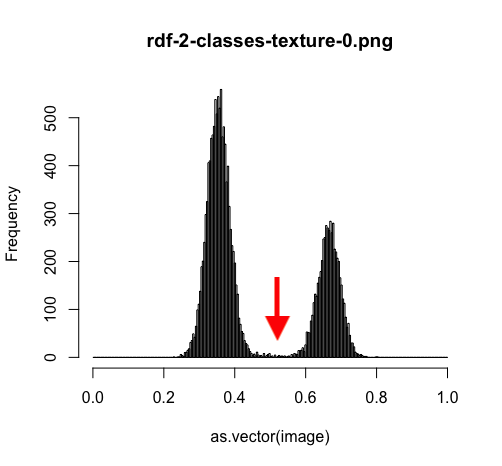
\includegraphics[scale=0.5]{threshold_explanation.png}
    \caption{Choosing the threshold}
    \label{fig-threshold-explanation}
\end{figure}

\begin{lstlisting}[language=R, caption=Segmenting based on the gray threshold]
    buildBinaryImage <- function(nom, threshold){
        image <- rdfReadGreyImage (nom)
        binaire <- (image - threshold) >= 0
        # a "trick" to make the error calculation more precise
        bin_1 = sum(binaire)
        bin_0 = dim(binaire)[1] * dim(binaire)[2] - bin_1
        if (bin_0 < bin_1)
            binaire = 1 - binaire
        
        # reference image
        reference <- rdfReadGreyImage ("rdf-masque-ronds.png")
        # results
        error = sum(binaire != reference) / (dim(reference)[1] * dim(reference)[2])
        error = round (error, 4) * 100
        info <- sprintf("%s\nthreshold=%s\nerror=%s%%", nom, threshold, error)
        if (interactive()){
            display (binaire, "image binaire", method="raster", all=TRUE)
            legend(x=0.5, y=dim(binaire)[2]/2, info, bg = "lightgreen", box.col = "lightgreen", yjust=0.5)
        }
    }
\end{lstlisting}

\paragraph{}
Observation: in the code above, we consider that the majority of pixels are for objects.
Therefore, if in our segmentation it's the opposite way, we reverse the image (lines 5-8) so we have a more precise error \footnote{The error represents the percent of missclassified pixels, relative to the reference image} calculation.

\clearpage

\paragraph{}
Taking a look at the results, we realise it was not incorrect to call this a \emph{simple} form of segmentation.
It's rather effective to reach about the same results as our reference image \ref{fig-reference-image} for the first 2 textures, having a low error.
However, for the last 2, we don't have a clear ``valley'' \ref{fig-threshold-explanation} in the histogram that we can use as our threshold.
For example, the histogram of the last texture resembles a Gaussian distribution, therefore the gray values are evenly distributed relative to their center: $\mu\approx0.5$.
\paragraph{}
As a result, we receive an error of about $50\%$ for the last texture when trying to somewhat resemble the reference image.
Our lowest error will be achieved by setting the threshold to either $0$ or $1$, but that will not help us at all.

\begin{figure}[h]
    \centering
    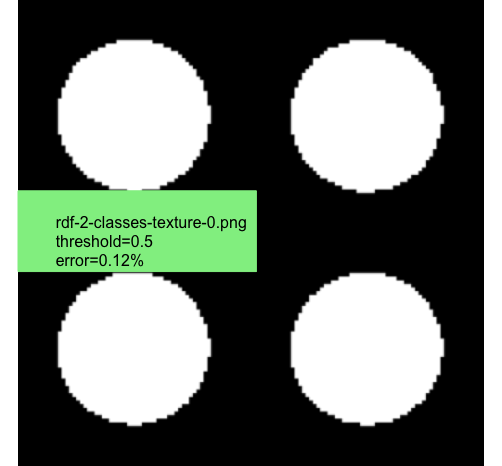
\includegraphics[width=\textwidth/3]{texture_0_threshold.png}
    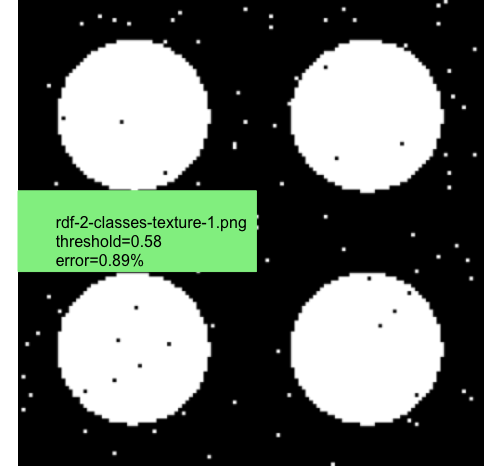
\includegraphics[width=\textwidth/3]{texture_1_threshold.png}
    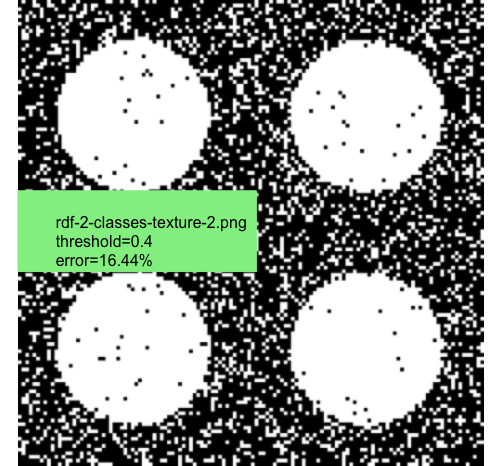
\includegraphics[width=\textwidth/3]{texture_2_threshold.png}
    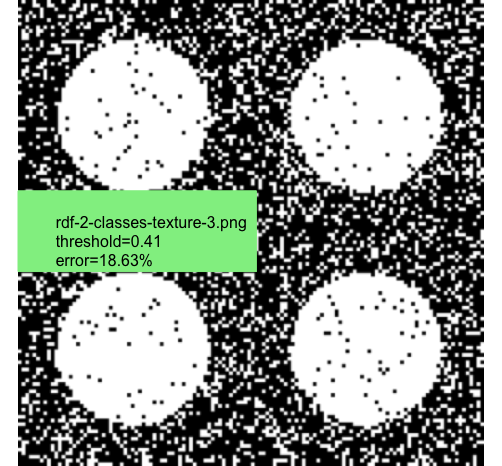
\includegraphics[width=\textwidth/3]{texture_3_threshold.png}
    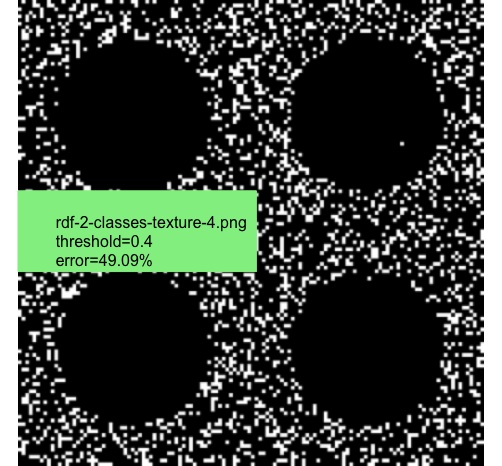
\includegraphics[width=\textwidth/3]{texture_4_threshold_1.png}
    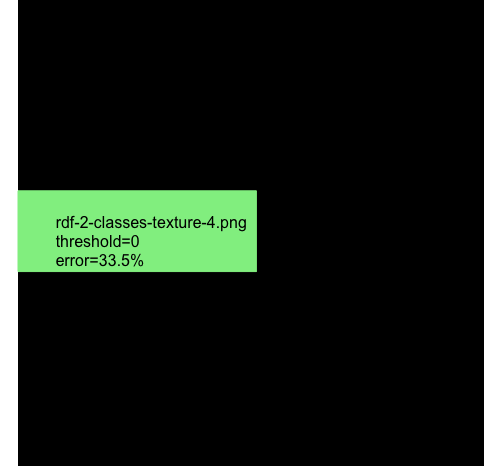
\includegraphics[width=\textwidth/3]{texture_4_threshold_2.png}
    \caption{Image segmentation based on gray threshold}
\end{figure}

\paragraph{}
We can conclude this experiment by saying that this method will not suffice, especially for ``noisy'' textures, as seen above.
Even for the simple textures we still have some missclassified pixels, as it's hard (or often times impossible) to get the right threshold for a perfect segmentation.
It is intuitive that the single white pixels (for example for the second texture) surrounded by black pixels should also be part of the background, so next we'll focus on trying to use a pixel's neighbours to gain more information.


\section{Texture levels}
\section{Histograms of texture levels}
\paragraph{}
We can define a pixel's \emph{texture level} as being the standard deviation of the gray levels for the pixels located in a square neighborhood.
Firstly, we select the \emph{neighbourhood size} we want to work with.
From there on, we'll just ``sweep a neighbourhood window'' over each pixel to calculate the average gray level.
This can be done with the help of fast 2D FFT convolution product, as described in the \emph{filter2()} function documentation.

\begin{lstlisting}[language=R, caption=Calculating the texture levels]
    # Moyennage d'une image
    rdfMoyenneImage <- function (image, taille) {
        # cote du masque = 2 *taille + 1
        taille <- 2* taille + 1
        masque <- array (taille ^ -2, c (taille, taille))
        # image filtree
        filter2 (image, masque)
    }

    # Ecart type normalise des voisinages carres d'une image
    rdfTextureEcartType <- function (image, taille) {
        # carre de l'image moins sa moyenne
        carre = (image - rdfMoyenneImage (image, taille)) ^ 2
        # ecart type
        ecart = sqrt (rdfMoyenneImage (carre, taille))
        # normalise pour maximum a 1
        ecart / max (ecart)
    }
\end{lstlisting}

\paragraph{}
The 